%%%%%%%%%%%%%%%%%%%%%%%%%%%%%%%%%%%%%%%%%%%%%%%%%%%%%%%%%%%%%%%%%%%%%%%%%%%%%%%%
% This is the Mamba user manual Tex source

\documentclass[a4paper,10pt,oneside]{article}
\usepackage[table]{xcolor}
\usepackage{mamba}

\title{Mamba Image User Manual}
\author{Nicolas BEUCHER \and Serge BEUCHER}
\date{\today}

%%%%%%%%%%%%%%%%%%%%%%%%%%%%%%%%%%%%%%%%%%%%%%%%%%%%%%%%%%%%%%%%%%%%%%%%%%%%%%%%
% Document

\begin{document}

\mambaCover
\mambaContent
\mambaFigures

\section{Introduction}

This document is the user manual of the library for Python \textbf{Mamba Image}.

Mamba Image is a mathematical morphology library, its name actually stands for 
\textbf{MA}thematical \textbf{M}orphology li\textbf{B}r\textbf{A}ry \textbf{Image} 
(For sake of simplicity, the library will be referred to as Mamba). The library 
provides a wide set of functions needed to perform common operations used in 
mathematical morphology like erosion, dilation, etc... but also more complex ones
(geodesic operators, watershed transformations...).

Before reading this document, make sure you have basic knowledge of Python
programming language (see the Python tutorial at 
\url{http://docs.python.org/tutorial/}) and that you know the basics of 
mathematical morphology (online courses are available at 
\url{http://cmm.ensmp.fr/~serra/acours.htm} and \url{http://cmm.ensmp.fr/~beucher/publi.html}).

This document addresses various points to help you understand how to use and
enjoy Mamba, such as getting familiar with it, what it does and doesn't,
understand how the library works, what you can do to optimize it for your
needs. If you are new to it, read the next section, quick start, before going
further.

\pagebreak

\section{A quick start}

For all intent and purpose, we will now assume that you know what mathematical
morphology is, at least theorically (and your interest in Mamba is to go 
practical), and that you have a minimum know-how in programming with Python.

We are aware that fulfilling these two conditions may be quite difficult. It is 
likely you know one and not the other. The present authors were unable to 
fulfil them when the project Mamba started. So don't get discouraged if you are
not yet familiar with one aspect or the other. There is plenty information over
the web to get you started on either one. This document is not intended to serve
as a mathematical morphology course nor as a programming lesson as these goals are
beyond our time or ability to perform. However, we list at the end of the
document (see appendix \ref{cha:to_go_further}) various websites or pdf documents which are 
accessible online that can provide you with this information. Of course, we hope that
Mamba will give you the incentive to learn one aspect or the other to solve
any image analysis problem you may have (see our examples to see the 
possibilities offered by such a tool).

To get started with Mamba, you need to install some software on your PC. The 
most obvious one is Python. You can find Python at \url{http://www.Python.org}. 
Download version 2.7 or 3.4 and install it. Once Python is installed, you will
need to download the lastest version of the Python Imaging Library (we
recommand you use the friendly fork pillow as we do use and test Mamba with it) at 
\url{https://pypi.python.org/pypi/Pillow/}.
You need to download the version corresponding to your version of Python (this
should be indicated in the name of the file). Again install it. On Linux, you may
have to install the Tkinter library if it was not provided with your Python
distribution (Windows users don't need to worry as it is part of the standard 
Python distribution they just installed). Finally download the Mamba library 
from \url{http://www.mamba-image.org} (as for PIL select the version corresponding
to your Python version) and install it.

These instructions may not be interpreted in the same way depending on your 
system specification. If you need more information refer to section
\ref{cha:inst_comp}.

At this point your PC is now equipped with every piece of software it needs to
use Mamba, so let's get started.

First, we will show you how to launch Mamba and use it in your programs.
To use Mamba, simply type in your Python console:

\lstset{language=Python}
\begin{lstlisting}
from mamba import * 
\end{lstlisting}

This import only gives you direct access to all the functions needed to 
perform basic and usual operations found in every mathematical
morphology algorithm.

The 3D operators can be accessed through the following import:

\lstset{language=Python}
\begin{lstlisting}
from mamba3D import *
\end{lstlisting}

\tipBox{
If you are using Windows, you can start more easily by clicking on the created
Mamba Shell shortcut in your start menu. It will launch an IDLE (the standard
Python shell on Windows) with preloaded mamba modules and packages and some 
default images created. If you are an IDLE user, this is the
recommanded way (see section \ref{cha:lim_restrict} for more information
regarding Mamba and IDLE).
}

You now have all the tools offered in Mamba loaded on your computer and you are
ready to try your ideas. Obviously you have some image that you would like to
process, so naturally the very first step is to load it into your program.

\lstset{language=Python}
\begin{lstlisting}
# Replace the "path/to/your/image" by the correct path
im = imageMb("path/to/your/image")
\end{lstlisting}

At this point, you can manipulate your image using the reference im. For example,
you could try to get some information about this image:

\lstset{language=Python}
\begin{lstlisting}
# Printing the size of the image (width, height)
print(im.getSize())
# Printing the depth of the image 
print(im.getDepth())
\end{lstlisting}

The first thing you may notice is that the returned image size is not the actual
image size (as it is registered when you look into the image properties). For
performance sake, Mamba can only work with images that have a width multiple of 64
and a height multiple of 2. If not, the image is automatically padded. You can 
also notice that your image was put into a greyscale image (the second command 
returns 8 which means 8 bits per pixel, the image pixels can take 256 values, from 
0 to 255). This is the default behavior for Mamba.

Well, this is all interesting but it does not give you access to the primary
properties of an image i.e. how it looks like. To do so, Mamba gives you access to
an embedded image displayer. You can call it for every image you create.

\lstset{language=Python}
\begin{lstlisting}
im.show()
\end{lstlisting}

This should have created a window displaying your image. There is no color
obviously because your image was transformed into a greyscale image upon loading.

The display comes with lots of options and possibilities to help you visualize
your image. More information can be found in section \ref{cha:disp_im}.

Now you have loaded your image, you are displaying it and you have access to 
some of its properties but one image is insufficient so you will have to create
other images to store your computation, compare, etc ... At this point you can
create them with the same properties as image im:

\lstset{language=Python}
\begin{lstlisting}
# Creating other images
im1 = imageMb(im)
im2 = imageMb(im)
im3 = imageMb(im, 1)
\end{lstlisting}

Here we created 3 new images with the same properties as our original image im.
Thus im1, im2 and im3 will have the same size as im. im1 and im2 also share 
the same depth as im (i.e. 8 bits per pixels) whereas im3 was created with a 
binary depth (1 bit per pixel as specified by the second argument). There are many
possibilities for creating new images, refer to section \ref{cha:create_im} for
more details.

You can activate the display for all of them as well. A window will be created
for each.

Now to give you an idea of how to use the functions of Mamba, we will now show
you a small example using the created images above.

\lstset{language=Python}
\begin{lstlisting}
# 1 - Computing the gradient of image im and putting the result in im1
gradient(im, im1)
# 2 - Computing a small opening of image im and putting the result in im2
open(im, im1)
# 3 - Computing the gradient of im2 and putting the result in im2
gradient(im2, im2)
# 4 - Converting im1 into binary and putting the result in im3
convert(im1, im3)
\end{lstlisting}

As random as these examples are (they are here for the sake of demonstration),
you may have already noticed some points. Firstly, function names closely
match the mathematical operators they are implementing (We tried to respect this
rule as best as we could to make the code more understandable). Secondly, you can
use an image both as input and output in the same function (see number 2). Last
but not least, convert is not the best function to transform your greyscale image into
a binary version at least from a mathematical morphology point of view.

And by the way, if you happened to have activated the display for the result
images, you may have found that the operations were quite slow (although in these 
basic examples, they are not so slow...). Indeed the 
display is automatically updated for each operation. Of course, when there is
only one (such as for convert) this is quite transparent but many functions, 
e.g. gradient and open, are a mix of other basic functions for which there is
a display udpate for every call. Let us assure you that the delay is only a
consequence of display updates.

\lstset{language=Python}
\begin{lstlisting}
# Activating the display and performing a size 100 erosion
im1.show()
erode(im, im1, 100)
# Now disabling the display and doing the same operation
im1.hide() # <- you can also close the window or minimize it
erode(im, im1, 100)
\end{lstlisting}

This example ends this very simple introduction to Mamba. Of course it does not
cover everything you can do with Mamba nor gives you all the details to better
harness its capabilities. However, hopefully now you have a basic understanding 
of how the library works. For more precision, read section \ref{cha:using_library}.
Also note that this document does not list the functions offered in Mamba, you
will need to refer to the Python reference document or to the Python API
quick reference for a list and explanations.

\pagebreak

\section{Why/When use Mamba?}

Before going further in this document, let's see why you should use Mamba and, 
almost more importantly, when. It can be sum up in the following sentence:

Mamba is meant to be a fast and easy library for coding mathematical morphology 
algorithms.

What we meant here is that, if your main concern is to try new algorithms to 
address your mathematical morphology problems while not waiting all night long 
for your result to come out or worse not come out because you made a mistake, 
then Mamba is meant for you. However, if you are looking for a library to perform
image processing tasks like convolutions, contrast enhancers or likewise, you 
had better not using it (try PIL instead). And by the way, Mamba does not make 
coffee (sorry about that...).

To do as intended, Mamba low level library is coded in C with performance through
simplicity in mind. The Python wrapper purpose is to give you an interface to 
that library which is fast to code and easy to play with (no compilation required 
and interactive help). Another objective regarding Mamba code is to be as 
portable as possible. This means that if you need to port your algorithm to a 
specific system you can easily adapt the C code to it.

Regarding licensing, Mamba is released under X11 license (also known as MIT 
license), see section \ref{cha:License} for more information.

To conclude this, let us remind you that mambas are fast-moving land-dwelling 
snakes of Africa. Their bite (at least for the black mamba) is extremely deadly 
but we assure you that no harm may come to you using Mamba... Well it won't bite
you.

\pagebreak

\section{License}
\label{cha:License}

Here is a copy of the license of Mamba. This license is known as the X11 license
(also named MIT license).

\vspace{0.5cm}

\begin{minipage}[c]{0.8\textwidth}%
 {\small Copyright (c) <2009>, <Nicolas BEUCHER and ARMINES for the Centre de 
 Morphologie Math\'{e}matique(CMM), common research center to ARMINES and MINES 
 Paristech>}{\small \vspace{0.5cm} \par}

{\small Permission is hereby granted, free of charge, to any person
obtaining a copy of this software and associated documentation files
(the \textquotedbl{}Software\textquotedbl{}), to deal in the Software
without restriction, including without limitation the rights to use,
copy, modify, merge, publish, distribute, sublicense, and/or sell
copies of the Software, and to permit persons to whom the Software
is furnished to do so, subject to the following conditions: The above
copyright notice and this permission notice shall be included in all
copies or substantial portions of the Software.}{\small \vspace{0.5cm} \par}

{\small Except as contained in this notice, the names of the above copyright 
holders shall not be used in advertising or otherwise to promote the sale, use 
or other dealings in this Software without their prior written authorization.}
{\small \vspace{0.5cm} \par}

{\small THE SOFTWARE IS PROVIDED \textquotedbl{}AS IS\textquotedbl{},
WITHOUT WARRANTY OF ANY KIND, EXPRESS OR IMPLIED, INCLUDING BUT NOT
LIMITED TO THE WARRANTIES OF MERCHANTABILITY, FITNESS FOR A PARTICULAR
PURPOSE AND NONINFRINGEMENT. IN NO EVENT SHALL THE AUTHORS OR COPYRIGHT
HOLDERS BE LIABLE FOR ANY CLAIM, DAMAGES OR OTHER LIABILITY, WHETHER
IN AN ACTION OF CONTRACT, TORT OR OTHERWISE, ARISING FROM, OUT OF
OR IN CONNECTION WITH THE SOFTWARE OR THE USE OR OTHER DEALINGS IN
THE SOFTWARE. }%
\vspace{1cm}
\end{minipage}

\warnBox{
Please note that this license does \textbf{\textsc{not}} cover documentation and
images found in source packages.
}

\pagebreak

\section{Requirements}
\label{cha:Requirements}

To use Mamba, you will need:
\begin{itemize}
\item A computer running Linux or Windows. Mamba will run on all kind of 
processors. However, you have to verify if yours supports SSE2 instructions. If you
are not sure, install the version of Mamba without SSE2, please note this version
is very slow. See \url{http://en.wikipedia.org/wiki/SSE2#CPUs_supporting_SSE2}
for a list of compatible CPUs.
\item Python version 2.7 or later (python 3 is supported).
\item Python Imaging library (pillow) for your current version of Python.
\item Tkinter (normally comes with Python on Windows systems but you may need to
install it on Linux systems).
\item VTK (optional, see \url{http://www.vtk.org/} for more info) with python
bindings if you want to use the mamba3D integrated display based on it.
\end{itemize}

\tipBox{
While Mamba3D will certainly work on a large range of systems, it is still
strongly recommanded that you work on a powerful computer if you want an
optimal experience with it (see section \ref{cha:perfo3D} for more information).
}

\pagebreak

\section{Installation/Compilation}
\label{cha:inst_comp}

\subsection{Windows XP/Vista/Seven}

If you are only interested in installing and don't want to go through the bother
of compiling it, just pick up the installer on the website. Select the appropriate
installer corresponding to you version of python (2 or 3, 32bit or 64bit), 
launch it and follow the instructions.

If you actually are interested in compiling the installers, here is the tools
you will need:

\begin{itemize}
\item Python version 2.7 or later with the distutils package.
\item SWIG version 2.0 or later (see \url{http://www.swig.org/}).
\item CMake version 2.8 or later (see \url{http://www.cmake.org/}) for the 
compilation process.
\item Microsoft Visual C++ Express 2008 or more recent (to compile you will then need
the stdint.h header. You can find it at 
\url{http://msinttypes.googlecode.com/svn/trunk/stdint.h}. Copy it in the VC/include 
directory of your Visual C++ installation).
\end{itemize}

Make sure you have correctly installed the required tools and that they appear
in your PATH environment variable. In particular, make sure that SWIG binary
(swig.exe) path is devoid of spaces as this may cause problems to the setup
script.

Get the source code of Mamba from the website. It comes in a zip that once
extracted will create a directory \textbf{Mamba.X.X}.

Launch CMake.

In \textit{"where is the source code"}, select \textbf{Mamba.X.X/src} with
the browse source button. Select a directory \textit{"where to build the binaries"}.
This is an out of source build so you must create and select a different
directory than the source. For the sake of example we will use
\textbf{mamba\_build} in the following instructions.

Press the configure button in CMake. You should something like figure \ref{fig:cmake_win}.

\begin{figure}
\centering
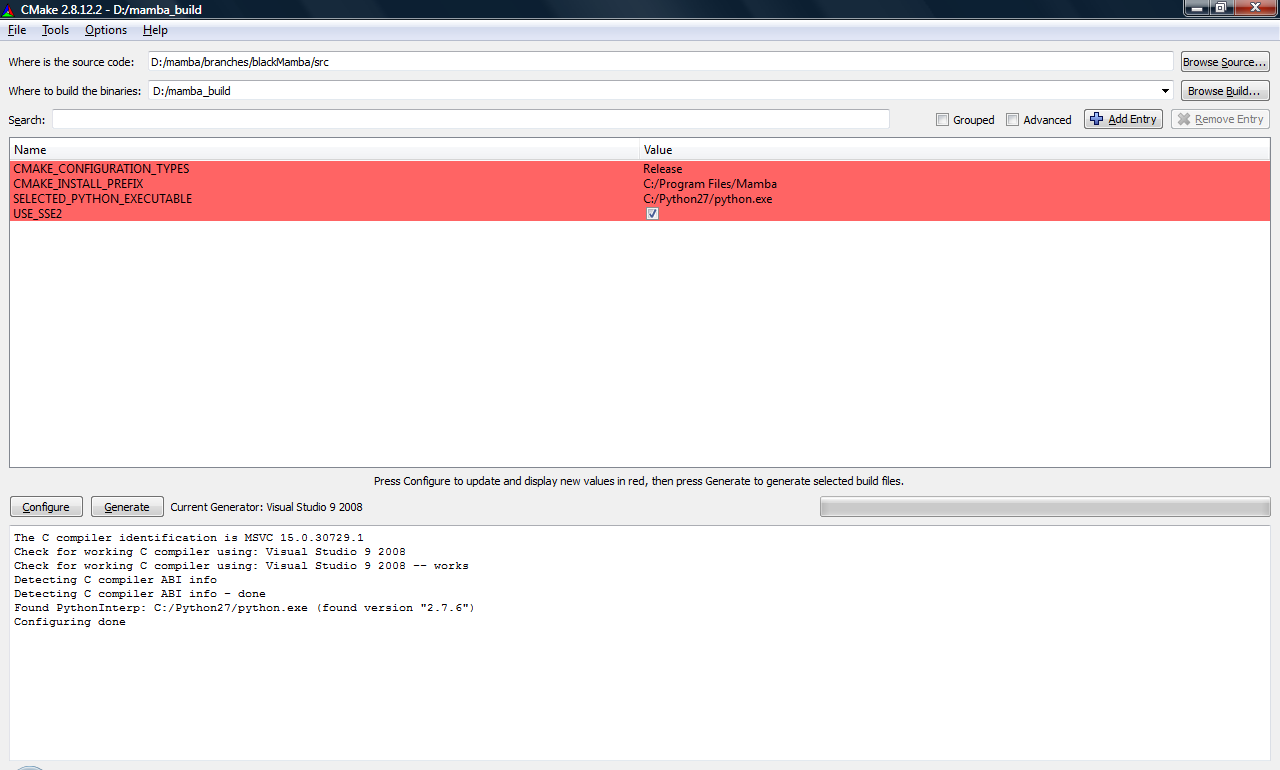
\includegraphics[scale=0.3]{images/cmake_win.png}
\caption{CMake configuration on Windows}
\label{fig:cmake_win}
\end{figure}

There are 4 configurable fields:
\begin{itemize}
\item \textbf{CMAKE\_CONFIGURATION\_TYPES}: Set this variable to "Release" to 
generate only the release configuration.
\item \textbf{CMAKE\_INSTALL\_PREFIX}: Ignore this option. It is a CMake 
mandatory that is not used by Mamba on windows.
\item \textbf{SELECTED\_PYTHON\_EXECUTABLE}: Make sure this option points 
to your python executable. In particular, if you have multiple python 
installation on your computer you should verify that you are using the 
correct one.
\item \textbf{USE\_SSE2}: Only on 32-bit systems, allows you to enable (default)
or disable SSE2 support in Mamba. On 64-bit systems, SSE2 is always enabled.
\end{itemize}

Once you have set the configuration, you must press Configure again for it to
take effect. Then press "Generate". This should have created a Mamba.sln file
in the \textbf{mamba\_build} directory.

Open this file using Visual C++, you should see something similar to figure
\ref{fig:visualcpp}.

\begin{figure}
\centering
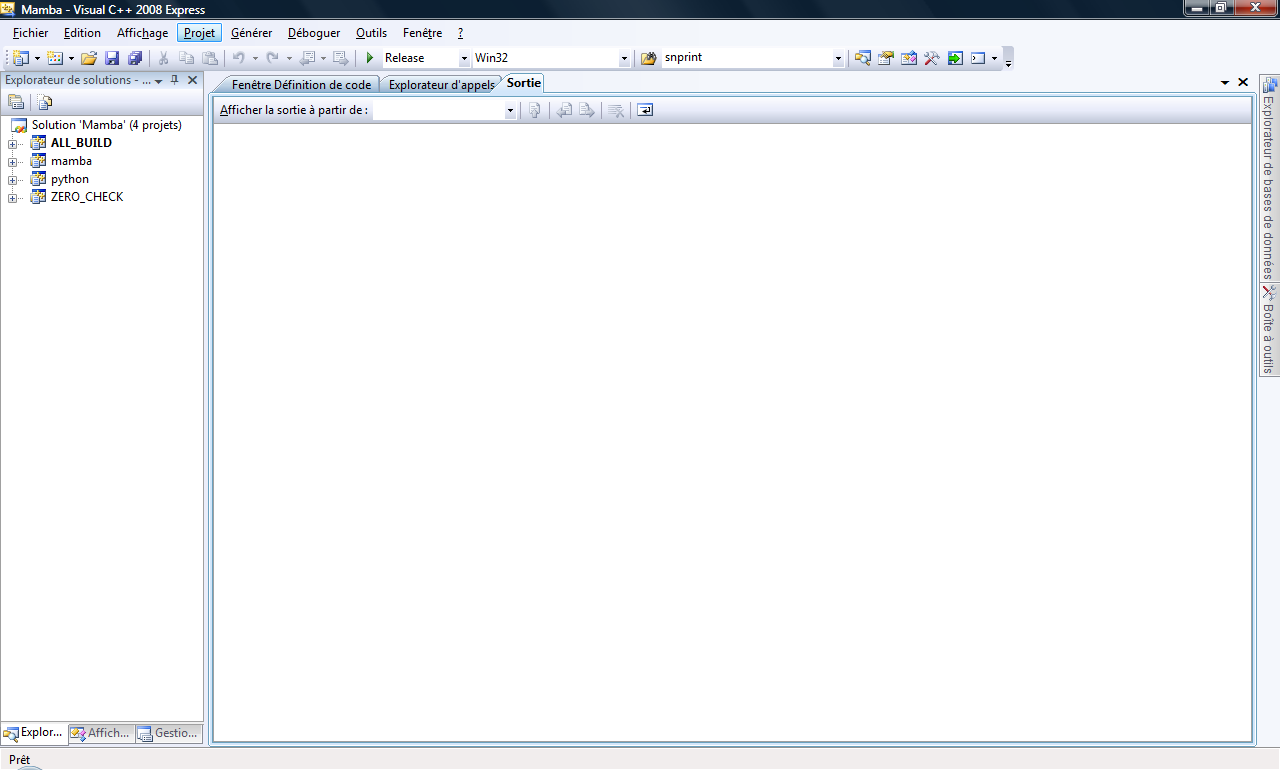
\includegraphics[scale=0.3]{images/visualcpp.png}
\caption{Visual C++ solution}
\label{fig:visualcpp}
\end{figure}

Open the menu \textit{"Generate"} and select \textit{"Generate ALL\_BUILD"}.
This should proceed with the compilation and the generation of the python installer.

If everything went OK, you should find in the \textbf{mamba\_build} directory
the following files:
\begin{itemize}
\item the python stand alone installer, Mamba Image-X.X.winYY-pyZ.Z.exe: in python/dist subdirectory.
\item C core library DLL (not needed for python): mamba.dll, mamba.def, mamba.lib in lib/Release subdirectory and includes files in include subdirectory.
\end{itemize}

We strongly recommand you verify the generated installer by installing it on
your computer and running the tests (see section \ref{cha:testing_mamba}).

\subsection{Linux}

Here are the command to type to compile and install on linux:

\texttt{cmake -C Mamba.X.X/src}\\
\texttt{cmake -D CMAKE\_BUILD\_TYPE:STRING=Release -D CMAKE\_INSTALL\_PREFIX:STRING=/usr .}\\
\texttt{cmake -G "Unix Makefiles" .}\\
\texttt{make}\\
\texttt{su -c "make install python\_install"}

\subsection{Other platforms}

If you are not running one the afore-mentionned systems but still want to try
Mamba, you will need to find how to do it on your own. Currently, we have only access to
these kind of systems and thus cannot provide you with instructions on how to do
it with others. However, the basic requirements and instructions will likely apply.

By the way, if you have installed Mamba on another platform (successfully!), please
share your knowledge with others. We will be happy to insert your procedure in this
user manual (and give you credits...).

\pagebreak

\section{Using the library}
\label{cha:using_library}

This section explains how to use the library.

\subsection{Philosophy and implicit working of the library}

Before giving you details regarding how to fully grasp the library, we would
like to give you details regarding the way it implicitly work. This section aims
at presenting some aspects that will always be present in Mamba but likely not 
explained nor talked about.

When we talk about an 'EMPTY' image or edge, this always means that pixels 
(inside or outside the image) take value 0. Thus an empty
image is an image where all the pixels are set to 0. On the opposite, the term 
'FILLED' is always associated with the maximum possible value of a pixel (which
depends on the image depth).

All image pixels are stored with unsigned integers. This is true for binary,
greyscale and 32-bit images.

As a consequence of the coding rules applied to Mamba, functions image parameters
always begin with the input arguments and ends with the output arguments (This 
is a general rule and there may be some exceptions for particular functions).
Most of the time, images arguments are imIn when the image is an input and imOut
when it is the output of the function. When functions require arguments other than 
image arguments (scalar values, edge or grid settings, etc.), they are placed after 
the image arguments.

When functions accept input and output images, you can safely use the same image
for both and you will obtain the expected result. If the function cannot 
guarantee this, it will return an error.

Regarding the Mamba3D package, it was created to be able to apply the same
algorithms developped for 2D images using Mamba to 3D images. To achieve
this goal, several choices
were made:

\begin{itemize}
\item Reuse as much as possible the basic C operators from Mamba to perform
the 3D computations to avoid rewriting them (Apart from hierarchical and
labelling operators this was actually possible).
\item Make sure functions and classes keep the same "look and feel" as their
counterpart in Mamba.
\item Provide an adapted display as there is one in Mamba.
\end{itemize}

These choices had consequences on the design of the package and thus on its
capacities. Overall we believe the possible downfall of that choices are
dimmed by the gains in terms of easiness of use, reuse of proven and robust
code and work versus objective ratio.

\subsection{A word for previous versions users}

Version 2 of Mamba introduced a lot of changes, made for performance and
easiness improvement, that \emph{will} break your scripts written for previous
versions (1.x). However we believe this should not present too much challenge
to upgrade your scripts to the newest version.

The list of changes is too big to be put here but here are the most obvious:
\begin{itemize}
\item mamba, mambaDraw, mambaExtra modules and the mambaComposed package have
been merged inside a single unified mamba package.
\item the former mamba3D addon is now part of the library.
\item the display methods names have been shortened.
\item some basic level functions have changed (in particular the neighboring
functions).
\item The C low level has been extensively reworked.
\end{itemize}

The result of these changes is a faster and, we hope, more user-friendly
library.

\subsection{Contents of the library}

The Python Mamba library is composed of three packages:
\begin{itemize}
\item mamba : which is the main package of mamba and contains all the operators
(from the most basic to quite advanced ones) to perform mathematical morphology
computations on 2D images.
\item mamba3D : which contains the same operators (save some of them without
equivalent in a three dimensional context) working on 3D images.
\item mambaShell : which is a container for functions and modules that are
needed to create and operate an appropriate shell for Mamba. In particular, it
contains demo presentations.
\end{itemize}

\subsection{Importing the packages}

To use Mamba, simply type in your Python console:

\lstset{language=Python}
\begin{lstlisting}
import mamba
\end{lstlisting}

This is the recommanded Python import method because it separates each package
or module you may use in its own name reference space. However this is quite painful
to work with when you are using Mamba in a console mode as all the function 
calls have to be preceded by

\lstset{language=Python}
\begin{lstlisting}
mamba.
\end{lstlisting}

So to avoid this, type:

\lstset{language=Python}
\begin{lstlisting}
from mamba import *
\end{lstlisting}

The later will give you direct access to the module functions and variables.

However, please note that some function names in mamba are more likely to
interfere badly with other Python packages, e.g. open and close functions. To 
avoid this, while not being forced to type "mamba." before each function 
name, the best way would be to import it via an alias to shorten its name:

\lstset{language=Python}
\begin{lstlisting}
import mamba as mb
\end{lstlisting}

If you want to use the 3D operators, the same recommendations apply for the
mamba3D package.
\lstset{language=Python}
\begin{lstlisting}
# You can pick up any import method you like
import mamba3D
from mamba3D import *
import mamba3D as mb3D
\end{lstlisting}

\subsection{Grid and Edge}

Grid and edge are important notions in mathematical morphology. Let us explain
how they are handled in Mamba. 

The edge defines the status of all the pixels which are not in the image. Let us 
explain what this assertion means. Obviously, any image is made of a finite set 
of pixels. However, mathematical morphology operations, which are neighbourhood 
operations, need that the status of the neighbour points of the pixels which are at 
the edge of the image be defined, otherwise it would not be possible to define the 
transformation. This is the purpose of the edge attribute. The edge defines the 
virtual pixels which are outside the image. The edge (remember, it is the outside 
edge) can be set to \textbf{empty} or 
\textbf{filled}. The \textbf{empty} edge is assuming that external world surrounding 
the image is made of virtual pixels at value 0 (the edge is set to 0) whereas 
the \textbf{filled} edge assumes an external world completely filled 
(the edge is set to the maximum possible value of a pixel according to the image 
depth). 

The grid defines the neighbourhood of each pixel in an image.

There are two possible grids in Mamba: \textbf{HEXAGONAL} or \textbf{SQUARE}. The 
\textbf{HEXAGONAL} grid defines six neighbours for each pixel as can be seen in 
figure \ref{fig:hxgrid}. The \textbf{SQUARE} grid defines the usual eight 
neighbours for each pixel as in figure \ref{fig:sqgrid}.

\begin{figure}
\centering
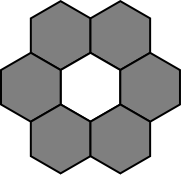
\includegraphics[scale=0.3]{figures/hxGrid.png}
\caption{Hexagonal grid}
\label{fig:hxgrid}
\end{figure}

\begin{figure}
\centering
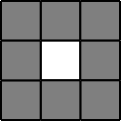
\includegraphics[scale=0.4]{figures/sqGrid.png}
\caption{Square grid}
\label{fig:sqgrid}
\end{figure}

As you will see later in this document, some functions need a direction or a 
neighbor as input. Figures \ref{fig:hxgriddir} and \ref{fig:sqgriddir} give you
the direction/neighbor encoding depending on the grid in use. The directions
are numbered from 0 to 6 or 8.

\begin{figure}
\centering
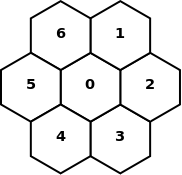
\includegraphics[scale=0.3]{figures/hxGriddir.png}
\caption{Directions on hexagonal grid}
\label{fig:hxgriddir}
\end{figure}

\begin{figure}
\centering
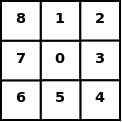
\includegraphics[scale=0.4]{figures/sqGriddir.png}
\caption{Directions on square grid}
\label{fig:sqgriddir}
\end{figure}

There are three possible grids in Mamba3D. You will
find they work the same as in Mamba except that they are a bit more
difficult to represent. We will try to give you an overview
of what they look like. Also they have some limitations that we think you
should be aware of.

As a foreword, we would like to explain how 3D grids are built in Mamba3D.
Instead of Mamba, where grids where defined for low-level C operators, Mamba3D
grids are very high level complex structures. They are built using 2D grids and
a mix of programmation magic. Some operators were rewritten in low-level C
functions working on 3D images because their 2D counterpart could not be adapted
to a 3D structure (e.g. hierarchical queues operators). As they work using the
grid, we defined some grids in low-level C but not all of them (too much work).
So some operators may not work with the grid you selected. Be warned !

\tipBox{
Grids in Mamba3D are strongly influenced by crystallography. For example,
the face centered cubic grid is describing the way carbon atoms are 
crystallized to form diamonds and centered cubic (also named body centered
cubic) is a structure by which iron atoms organise themselves. Of course, there
is a lot of other structures in crystals that are not represented in Mamba3D.
}

Here are the Mamba3D grids (the figures representing the grids are projections,
they indicates directions/neighbors numbers):

\begin{itemize}
\item \textbf{CUBIC}: The very basic cubic grid, built by stacking square
grids one on the other. See figure \ref{fig:cubic_grid}.

\begin{figure}
\centering
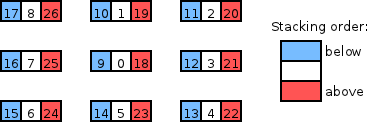
\includegraphics[width=0.55\textwidth]{figures/cubic_grid.png}
\caption{Cubic grid}
\label{fig:cubic_grid}
\end{figure}

\item \textbf{FACE\_CENTER\_CUBIC}: A face centered cubic grid. It is in fact
built by stacking hexagonal grids one on the other with a slight shift. See
figure \ref{fig:fcc_grid}.

\begin{figure}
\centering
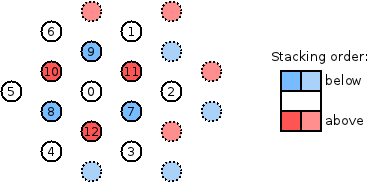
\includegraphics[width=0.55\textwidth]{figures/fcc_grid.png}
\caption{Face centered cubic grid}
\label{fig:fcc_grid}
\end{figure}

\item \textbf{CENTER\_CUBIC}: Known as the body centered cubic, this grid is
built by stacking square grids with a half shift in the two directions. See
figure \ref{fig:ccubic_grid}. This grid is not supported by low-level C
operators.

\begin{figure}
\centering
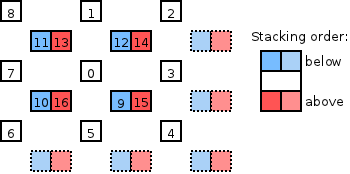
\includegraphics[width=0.55\textwidth]{figures/ccubic_grid.png}
\caption{Centered cubic grid}
\label{fig:ccubic_grid}
\end{figure}

\end{itemize}

As it is, we could have added a lot more grids in Mamba3D. For example,
we could have built a grid stacking without any shifted hexagonal grids.
We chose not to do it, but it does not mean you can't, although we doubt very
much you find such grids useful. In this event, we encourage you to look
at section \ref{cha:create_grid3D}.

Regarding the FACE\_CENTER\_CUBIC, you can notice on figure \ref{fig:fcc_grid}
that the triangles drawn by below directions (blue) and above directions (red)
do not point the same way. This is very important to be able to draw a 
cuboctahedron instead of an anti-cuboctahedron.

Be aware that the grid is never an image attribute, but a structuring element 
attribute. A structuring element is always defined on a given grid. Therefore, 
when performing a transformation with a given structuring element, the corresponding 
grid will be used with the image. Changing the grid of an image can be seen as a 
simple shift of the even lines of the image versus the odd ones so that the pixels 
belonging to an even line are between the pixels of the following odd line. The even 
lines are shifted to the right compared to the odd ones (the first line is numbered 0, 
it is therefore an even one).

By default, when it is launched, Mamba uses the \textbf{HEXAGONAL} grid (through 
the DEFAULT\_GRID variable). Mamba3D uses the \textbf{FACE\_CENTER\_CUBIC} grid
(through the DEFAULT\_GRID3D variable)  Each function requiring a grid
configuration as a parameter is given DEFAULT\_GRID(3D) by default. When an
edge status is needed, the default value is selected depending on the operator
in use. The edge, as the grid, is not an image attribute.

There are different ways to change the grid. Firstly, you can use the setDefaultGrid 
(setDefaultGrid3D for Mamba3D) function:

\lstset{language=Python}
\begin{lstlisting}

# Changes the default grid (DEFAULT_GRID) to HEXAGONAL
setDefaultGrid(HEXAGONAL)

# Changes the default grid (DEFAULT_GRID) to SQUARE
setDefaultGrid(SQUARE)
\end{lstlisting}

Secondly, you can do nothing and let some functions do the job for you!

You can get a list of all the available directions given the grid that is in use
by calling the function getDirections (getDirections3D for Mamba3D).

\lstset{language=Python}
\begin{lstlisting}
# Returns a list of all the available directions for the default grid
directions = getDirections()
# Returns a list of all the available directions for the SQUARE grid
directions = getDirections(SQUARE)
# Returns a list of all the available directions for the HEXAGONAL grid
directions = getDirections(HEXAGONAL)
\end{lstlisting}

There are other utilities functions that are provided by Mamba and Mamba3D to
handle  directions/neighbors. Refer to the Python API reference.

\subsection{Creating and manipulating 2D images}
\label{cha:create_im}

\paragraph{Creating images}

To handle images, a Python class named imageMb has been created. This class will allow
you to create, load, save and perform standard operations on your images.

The imageMb constructor offers a wide range of possibilities to create an image. 
Here is the list of all these possibilities:

\begin{itemize}
\item \texttt{\textbf{imageMb()}}: without arguments will create an empty 
greyscale image.
\item \texttt{\textbf{imageMb(im)}}: will create an image using the same size 
and depth than 'im'.
\item \texttt{\textbf{imageMb(depth)}}: will create an image with the desired
'depth' (1, 8 or 32).
\item \texttt{\textbf{imageMb(path)}}: will load the image located in 'path'.
\item \texttt{\textbf{imageMb(im, depth)}}: will create an image using the same 
size than 'im' and the specified 'depth'.
\item \texttt{\textbf{imageMb(path, depth)}}: will load the image located in 
'path' and convert it to the specified 'depth'.
\item \texttt{\textbf{imageMb(width, height)}}: will create an image with size 
'width'x'height'.
\item \texttt{\textbf{imageMb(width, height, depth)}}: will create an image with
size 'width'x'height' and 'depth'.
\end{itemize}

When not specified, the width and height of the image will be set to 
256x256. The default depth is 8 (greyscale).

For performance sake, Mamba works only with images that have a width multiple of
64 and a height multiple of 2. It means that if you requested the creation of
an image of size 360x201, Mamba will actually create an image of size 384x202. 
The actual image is always larger than or equal to the defined size.

There is a size limitation when you define images. This limitation is given by
the number of pixels in the image which must be lower than or equal to $2^{32}$.
This is a really huge value which allows you to define 65536x65536 images for instance.
A 200000x10000 image is also allowed (number of pixels lower than the limit).
Note however that, in practice, the real allowed maximum size is smaller as you would
need a fairly huge amount of memory to handle these images in Mamba. So, be sure
that your memory space is sufficient if you intend to use big images.

When loading an image from a file, please note that Mamba accepts all 
kinds of images (actually all the PIL supported formats). You can specify
the RGB filter that will be used to convert color image into greyscale 
image by adding the rgbfilter=<your\_filter> to the argument of the
constructor (see PIL documentation for examples of filters).

\tipBox{
Mamba allows you to create images with different sizes but not to perform
computations between them. If you want to do so, you will have to use the
cropCopy() function to extract the part of the images you want to match.
}

\paragraph{Saving and loading images}

Once you have created an image and performed some operations on it, you may want 
to save it into a file. The imageMb class provides the method save() to do so:

\lstset{language=Python}
\begin{lstlisting}
# Saving the content of im1 image in test.png
im1.save('test.png')
\end{lstlisting}

The method uses PIL functions to save the image. Thus the format (bmp, gif, 
jpeg, ...) is automatically deduced from the extension used.

If you want to load an image into your imageMb object (assuming you did not make
it at the image creation) you can use the method load() to do so:

\lstset{language=Python}
\begin{lstlisting}
# Loading the content of test.png in image im1
im1.load('test.png')
\end{lstlisting}

Loading an image after the creation will not change the size of the original 
image to adapt it to the loaded image. The loaded image is padded/cropped to fit
the original size.

\paragraph{Other imageMb methods}

Besides creating, loading or saving your image, a range of other functionalities
are accessible using specific methods.

If you need to convert an image into another format (another depth), use the 
convert() method. Supported conversions are binary to greyscale (1->8) or 
greyscale to binary (8->1). A binary image is converted to a greyscale image using
0 for false and 255 for true. A greyscale image is converted to binary using the
following method: every pixel that is equal to 255 is set to true, otherwise 
false. convert() takes the required depth as argument. This method is here for 
convenient purposes, there are more elaborated ways to convert an image provided
inside Mamba.

\lstset{language=Python}
\begin{lstlisting}
# Converts the greyscale image into binary format
greyscale = imageMb(depth=8)
greyscale.convert(1)

# Converts the binary image into greyscale format
binary = imageMb(depth=1)
binary.convert(8)
\end{lstlisting}

If you want to erase an image, you can use the reset() method. 

\lstset{language=Python}
\begin{lstlisting}
# Erase the image im1 by setting all its pixels to 0
im1.reset()
\end{lstlisting}

The fill() method allows you to set all the pixels of an image to a given value.

\lstset{language=Python}
\begin{lstlisting}
# Fill im2 image with the value 3
im2.fill(3)
\end{lstlisting}

There are other methods that will be explained more thoroughly in the next sections.

\subsection{Creating and manipulating 3D images}

The basic data model used in Mamba3D is the image3DMb image class.

This class is derived from the sequenceMb class in the mambaComposed package.
You should know that this class is actually a stack of standard Mamba images
(imageMb object) with all the same size and depth. The dimension of a 3D image
is thus given by the size of the mamba images inside the stack and by its
length. This choice may seem strange because it differentiates one direction
(supposedly z-axis) in the data structure from the other two (x-axis and
y-axis) but it was dictated by the need to reuse as much as possible the 
basic C functions of Mamba which work with imageMb low-level structure.

There is a wide range of possibilities to create a 3D image object :
\begin{itemize}
\item \texttt{\textbf{image3DMb()}} : without arguments will create an empty
greyscale 3D image (by default its size is 256x256x256).
\item \texttt{\textbf{image3DMb(im3D)}} : will create a 3D image using the
same width, height, length and depth than 3D image 'im3D'.
\item \texttt{\textbf{image3DMb(im)}} : will create a 3D image using the same
width, height and depth than 2D image 'im' (a imageMb object). Its
lenght will be defaulted to 256.
\item \texttt{\textbf{image3DMb(depth)}} : will create a 3D image with the
desired 'depth' (1, 8 or 32) and default size (256x256x256).
\item \texttt{\textbf{image3DMb(path)}} : will load the image sequence located
in 'path', see the load method.
\item \texttt{\textbf{image3DMb(im3D, depth)}} : will create a 3D image using
the same size than 3D image 'im3D' and the specified 'depth'.
\item \texttt{\textbf{image3DMb(im, length)}} : will create a sequence using
the same width, height and depth than 2D image 'im' (a imageMb object). Its
length will be the specified 'length'.
\item \texttt{\textbf{image3DMb(path, depth)}} : will load the image sequence
located in 'path' and convert it to the specified 'depth'.
\item \texttt{\textbf{image3DMb(width, height, length)}} : will create a 
greyscale 3D image with 'width', 'height' and 'length'.
\item \texttt{\textbf{image3DMb(width, height, length, depth)}} : will create
a 3D image with the given parameters.
\end{itemize}

Refer to the Python reference manual of Mamba to get more info about the 
sequenceMb class. Specific 3D image methods information can be found in the
Mamba3D Python reference. In particular, image3DMb class defines a method
to load raw 3D data.

\subsection{Pixels manipulation}

The imageMb class offers three methods to set or get pixels in the image.

\lstset{language=Python}
\begin{lstlisting}
# Setting the pixel at x,y in im2 to value
position = (x,y)
im2.setPixel(value, position)
# Same as previously but this method will not update the screen
im2.fastSetPixel(value, position)
# Getting the pixel value at position
value = im2.getPixel(position)
\end{lstlisting}

\subsection{Color palette}

Color palette defines the way a grey pixel will be converted to color. It 
associates for each possible value (0-255) a tuple of values describing the red, 
green and blue components (R, G, B) of the wanted color. The final palette is 
built by concatenating all these tuples into a single one.

Mamba comes with three predefined palettes:

\lstset{language=Python}
\begin{lstlisting}
# The rainbow colors (0 equals black)
rainbow

#The inverted rainbow colors (0 equals white)
inverted_rainbow

#The patchwork colors (0 equals black), used mainly to
#better visualise mosaic images
patchwork
\end{lstlisting}

You can see the results of using these palettes in figure \ref{fig:palette}.

\begin{figure}
\centering

\includegraphics[scale=0.3]{images/test_ramp.png}
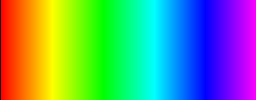
\includegraphics[scale=0.3]{images/test_ramp_r.png}
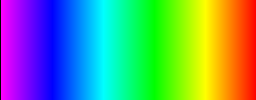
\includegraphics[scale=0.3]{images/test_ramp_ir.png}
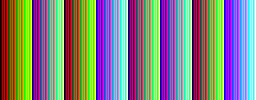
\includegraphics[scale=0.3]{images/test_ramp_p.png}
\caption{Effects of the rainbow, inverted rainbow and patchwork palettes on the first 
image}
\label{fig:palette}
\end{figure}

To apply or disable a palette to your image, use the following methods:

\lstset{language=Python}
\begin{lstlisting}
# Indicates that im1 will use palette as a color conversion
# table for display 
im1.setPalette(palette)

# Reset any palette conversion (the image will return to greyscale display)
im1.resetPalette()
\end{lstlisting}

When you apply a palette to an image, it will affect its display and the image 
stored by saving. The computations are not impacted. Be also aware that, if you 
save your image in color, you may have different values when reopening it with 
Mamba as the color to grey scale converter is not using your palette.

\subsection{Displaying 2D images}
\label{cha:disp_im}

When trying new algorithms, it can be very useful to be able to follow the 
evolution of your images without having to save the image at each step. Mamba
provides a graphical interface, see figure \ref{fig:win}, which can display 
every required image into its own display window.

To activate a display, type:

\lstset{language=Python}
\begin{lstlisting}
# Shows the image im in its own window
im.show()
\end{lstlisting}

\begin{figure}
\centering
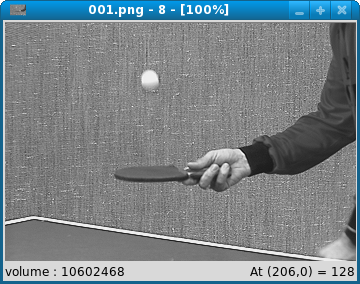
\includegraphics[scale=0.5]{images/mamba_win.png}
\caption{Image displayer window}
\label{fig:win}
\end{figure}

Every modification on this image will then be shown inside the opened window.
This operation is known to be very demanding on performance. The display also
gives information regarding the image volume, the position of the mouse inside
the image (and the pixel value associated).

There are numerous possibilities to control the display, here is the list of
keys and controls available inside the display:

\begin{itemize}
\item \textbf{P}: will dynamically (de)activate the color palette (provided you
attach one to your image using the setPalette() method).
\item \textbf{<Control-V>}: will copy any image stored inside the clipboard 
in your image (only works on Windows platforms).
\item \textbf{<Control-F>}: will freeze/unfreeze the display. See freeze() 
method below.
\item \textbf{<Control-R>}: will reset the display to its original size and 
zoom value.
\item When zoom value allows it, you can grab the image using your mouse by
holding the left button down and moving it.
\end{itemize}

\begin{figure}
\centering
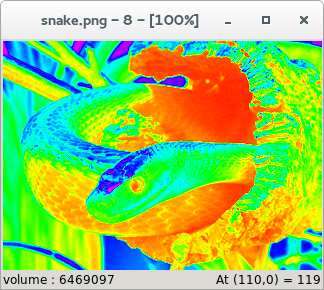
\includegraphics[scale=0.5]{images/mamba_menu.png}
\caption{Contextual menu}
\label{fig:menu}
\end{figure}

A contextual menu is also available by right-clicking in the display. It offers
services like saving, opening, etc. Figure \ref{fig:menu} shows an example of 
contextual menu. The first three choices are obvious. Then, you can choose a zoom
value between 100\% or 200\%. Interpolation is the way image will be processed
before being displayed when zoom value is different than 100\%. The choice
may affect the speed of display (for more information regarding the interpolation
methods, refer to PIL documentation). The last menu item indicates the size of
the image.

If you want to disable the display you have two options, either close the window
by clicking the appropriate button or type:

\lstset{language=Python}
\begin{lstlisting}
# Hide the window associated with im
im.hide()
\end{lstlisting}

Both operations will prevent the display to be updated for every modification of
the image and thus will remove the performance overhead (reducing or minimizing 
the display window will have the same result for performance but the window will
remain visible in your access bar).

If you want to stop the display from being automatically updated when a 
computation is performed while still being able to see it, you can freeze the 
display using the appropriate method:

\lstset{language=Python}
\begin{lstlisting}
# Freeze the window associated with im (no more updated)
im.freeze()

# Unfreeze the window associated with im (updated again)
im.unfreeze()
\end{lstlisting}

Sometimes, you will have lots of images opened and displayed making it quite
messy on your desktop and thus very difficult to read and analyze. There are a
bunch of methods and functions to help you organise your displays.

Firstly, you can give a name to your image that will be displayed in the window
title making it easier to know what is represented by the display:

\lstset{language=Python}
\begin{lstlisting}
# Setting im name to 'result'
im.setName('result')
\end{lstlisting}

When the screen gets filled with lots of displays it can be excruciatingly
boring and slow to order all of them so that they don't overlap. To make sure 
displays are properly and automatically organised you can call the following 
function:

\lstset{language=Python}
\begin{lstlisting}
tidyDisplays()
\end{lstlisting}

The function does not do miracles (like increasing your screen resolution) so
don't have too much expectations.

Large and small images are not displayed at their original size but they are
zoomed in (if they are too small) or zoomed out (if they are too large). By
default, images larger than 400 in width or height are zoomed out by a factor 2
until the size of the zoomed out displayed image is below this maximum value.
In the same way, an image smaller than 200 will be zoomed in (x2) until
the displayed image is larger than this minimum. For instance, a 1024x1024 image
will be displayed after a zoom-out equal to 25\% whereas a 200\% zoom-in will be
applied on a 128x128 image.

The default values of the display sizes can be changed by means of the following
functions:

\lstset{language=Python}
\begin{lstlisting}
setMaxDisplay(size)
setMinDisplay(size)
\end{lstlisting}

where size is a tuple containing the upper (in setMaxDisplay) or lower (in
setMinDisplay) limits of the width and height of the display.
These functions belong to the mambaDisplay module. It is wise to use them at
start before displaying any image. Under Windows, these functions could be put
in the \_init\_.py file of the Mamba shell (see section \ref{cha:mamba_shell}).

\lstset{language=Python}
\begin{lstlisting}
# Setting display max size to (800,800)
import mambaDisplay
mambaDisplay.setMaxDisplay((800,800))
\end{lstlisting}

\textbf{Important notice}: We saw previously that two grid definitions were 
available in Mamba: hexagonal or square grids. However, any image will always be 
displayed on a square grid, even if this image has been obtained with an operator 
defined on the hexagonal grid! Remember: the grid is an operator attribute, not an 
image attribute. This may lead to some strange phenomenons if you are displaying 
small hexagons for instance. They seem to be distorted and in fact they are. However, 
be sure that it's only a display artefact: the operator is really applied on an hexagonal 
grid (as you may ascertain this by displaying larger hexagons).


\subsection{Displaying 3D images}
\label{cha:disp_im3D}

As for basic Mamba images, 3D images can be displayed each individually with
their own window, see figure \ref{fig:dis3D_base}. Mamba3D offers by default
two possibilities to display 3D images and enables you to define your own
display. Mamba3D allows you to active multiple displays for one image.

\tipBox{
The foot data used for the display demo in this section can be found at
\url{http://tc18.liris.cnrs.fr/code_data_set/3D_images.html}
}

\subsubsection{Volume rendering display}
This display is ensured through the VTK library. This is the default display
if you have VTK (with Python bindings) installed on your computer.

To activate the volume display, type:

\lstset{language=Python}
\begin{lstlisting}
# Shows the 3D image in its own window
im3D.show()
# The previous call worked because VTK is the default display method
# you can explicitly ask for it
im3D.show("VTK")
\end{lstlisting}

\begin{figure}
\centering
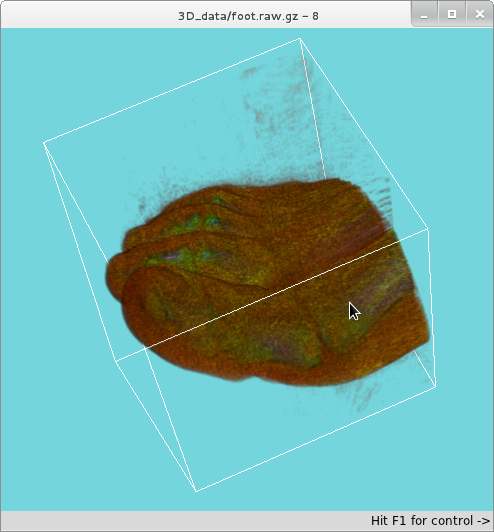
\includegraphics[scale=0.5]{images/display_base.png}
\caption{Image volume displayer window}
\label{fig:dis3D_base}
\end{figure}

The image is displayed inside its bounding cube and you can control its rotation
and zoom with your mouse.

The display comes with an integrated controller which allows you to change
the various options of display available. As shown in figure \ref{fig:dis3D_ctrl},
you can change the opacity, the background color and the rendering methods.

The transparency/opacity of a pixel depends on its value. By clicking on the 
transparency bar, every pixel with value below will be transparent and above
pixels will be opaque. You can also change the opacity by calling the 
appropriate method:

\lstset{language=Python}
\begin{lstlisting}
# Sets the opacity in reverse of default opacity (but let value 0 stay 
# fully transparent)
l = range(255,-1,-1)
l[0] = 0
im3D.setOpacity(l)

# Resetting the opacity to its default value
im3D.resetOpacity().
\end{lstlisting}

The color transfer function works the same as for the mamba images. In fact, you
must call the same method with the same kind of parameters.

\lstset{language=Python}
\begin{lstlisting}
# Indicates that im3D will use palette as a color transfer function
im3D.setPalette(palette)

# Resets any palette conversion (the image will return to greyscale display)
im3D.resetPalette()
\end{lstlisting}

To change the background, just click on the background bar. It will open a
color chooser dialog box in which you can pick up any background color you
might want.

\begin{figure}
\centering
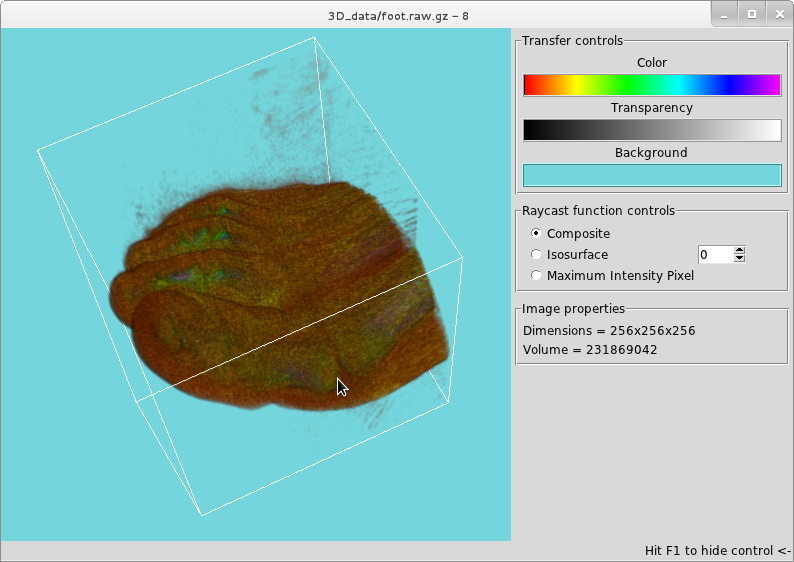
\includegraphics[scale=0.5]{images/display_ctrl.png}
\caption{Volume display controls}
\label{fig:dis3D_ctrl}
\end{figure}

Mamba 3D uses volume rendering techniques to display the data. VTK provides
three distinctive methods to perform volume rendering :
\begin{itemize}
\item \textbf{Composite} : the result is a blend of all the pixels crossed by
the ray of light accordingly to their color and transparency.
\item \textbf{Isosurface} : the result shows only pixels with a given
value. It also use shading to allow a better visualisation of the volume.
\item \textbf{Maximum Intensity Pixel (MIP)} : the result is the color and
transparency of the pixel with the highest value that the light ray hit.
\end{itemize}
You can see the results of the 3 different methods in figure 
\ref{fig:dis3D_method}.

\begin{figure}
\centering
\begin{tabular}{ccc}
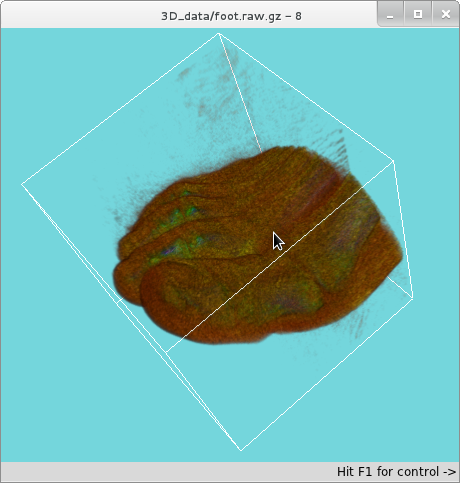
\includegraphics[width=0.25\textwidth]{images/display_compo.png} & 
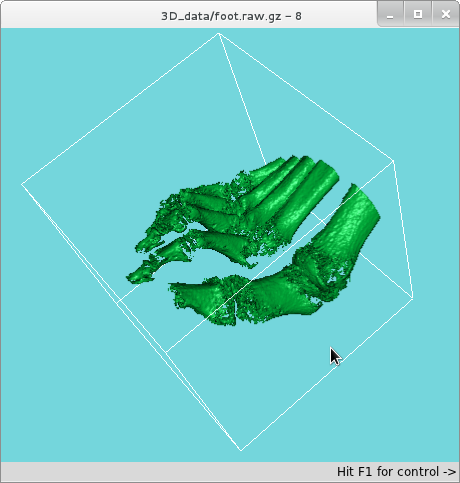
\includegraphics[width=0.25\textwidth]{images/display_isosurface.png} &
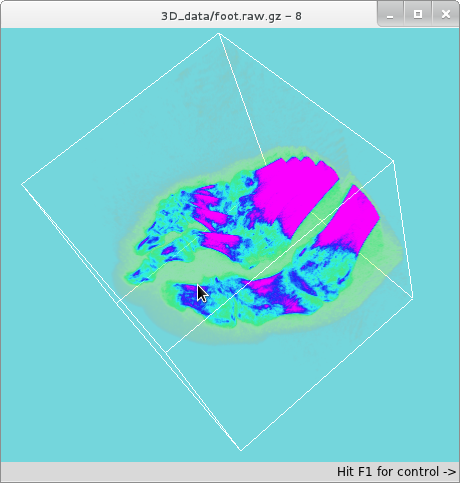
\includegraphics[width=0.25\textwidth]{images/display_mip.png} \\ 
Composite &
Isosurface &
MIP \\ 
\end{tabular}
\caption{Volume rendering techniques}
\label{fig:dis3D_method}
\end{figure}

You can rotate (holding your mouse left button while moving it), zoom in and
out (same movement while holding the right button) and displace the image
(this time by holding both the left button and the shift key on your keyboard
while moving the mouse). This allows you to view more precisely any area of
your image. You can restore the initial settings by pressing r (Although this
does not seem to affect rotation).

We feel this display is appropriate to get an overall idea of your
result. However, it may lack precision and it could be troublesome to
understand what or where you are looking at. Use it cautiously.

\subsubsection{Projection display}
This display is basically an adaptation of the 2D display available in Mamba.
It is a basic plane projection along the three axis.

To activate the volume display, type:

\lstset{language=Python}
\begin{lstlisting}
# Shows the 3D image in its own window using projection along axis
# Note that if you have opened a VTK display this new one will not
# replace it (you will now have 2 displays available).
im3D.show("PROJECTION")
\end{lstlisting}

\begin{figure}
\centering
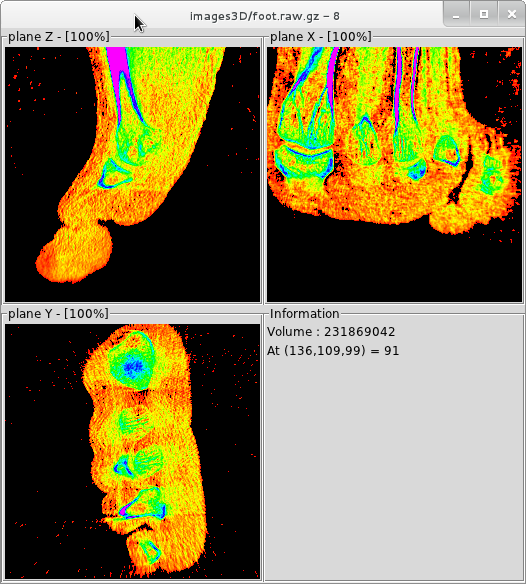
\includegraphics[scale=0.5]{images/display_proj.png}
\caption{Image projection displayer window}
\label{fig:dis3D_proj}
\end{figure}

You can navigate through planes moving your mouse while holding <ctrl> down.
The mouse motion will allow you to change the plane following it (the displayer
shows a red cross to indicate where you are in the image data).

This display does not support opacity tuning. However you can use a color
palette (same procedure that for VTK display).

This is a more appropriate display if you need precision and careful
analysis of a result. However it only shows a limited amount of the
image at any given time.

\subsubsection{3D displays particularities}
As you will see, unlike 2D images displays that are updated as the computations
progress, 3D images displays are not (for performance reasons). You will have
to update them manually by either hitting key <F5> on your keyboard (with
the focus on the display you want to update) or call the appropriate method
when you need an update:

\lstset{language=Python}
\begin{lstlisting}
# Updates the display
im3D.update()
\end{lstlisting}

We tried to provide Mamba3D with a coherent, useful and appropriate display.
However, contrary to 2D images, 3D images are difficult to represent on a 2D
display. Be sure to correctly configure the display before analysing results.
We do not believe Mamba3D display will fit all situations and you are
encouraged to look at other possible ways to display your data if you
think the one in Mamba3D in not good for you (refer to section \ref{cha:create_own_disp}
to get an idea of how to create your own display and use it).

Lastly, as 3D images in Mamba3D are stacks of 2D images (imageMb objects) you 
always have the possibility to activate their own display at all time.

\lstset{language=Python}
\begin{lstlisting}
# Activates the display for slice number 128 of 3D image
im3D[128].show()
\end{lstlisting}

\subsection{Structuring elements}

Two of the most important operations of mathematical morphology: erosion and
dilation (functions erode and dilate and their 3D counterpart respectively)
are based on a structuring element which controls the behavior of the operator.

The class structuringElement allows you to describe a structuring element to
be used with the erode and dilate functions. This class can only describe
structuring elements that are included in the local 
neighbors of the central point (adjacent points).

\begin{figure}
\centering
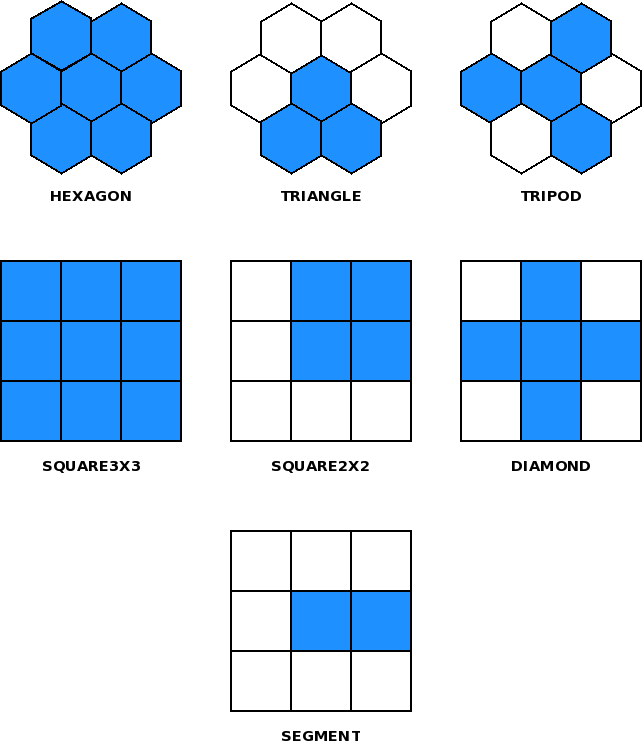
\includegraphics[scale=0.3]{figures/se.png}
\caption{Structuring elements defined in Mamba}
\label{fig:se}
\end{figure}

Mamba includes some of the most usual structuring elements. Figure
\ref{fig:se} gives their list and representation.

You can define your own structuring element easily. To do so you will need to
identify the grid it is based on and the points that you want to include 
inside your structuring element. Refer to figures \ref{fig:hxgriddir} and 
\ref{fig:sqgriddir} for neighbors coding values. Here is an example:

\lstset{language=Python}
\begin{lstlisting}
# Creating a reverse triangle
reverse_triangle = mambaComposed.structuringElement([0,1,6], mamba.HEXAGONAL)

# performing an erosion with the created structuring element
mambaComposed.erode(imIn, imOut, 1, se=reverse_triangle)
\end{lstlisting}

\warnBox{
Some erosion and dilation functions implemented in Mamba do not use this
structuring element class for performance or feasability reasons.
}

\warnBox{
Be also aware that when you are combining operations using a structuring element
and operations using a grid you may have discrepancies between the structuring
element internal grid and the grid you used as an argument (or the default). To
prevent this, use the getGrid() method of the structuring element class.
}

Mamba3D predefined four structuring elements to be used with the appropriate
3D operators:

\begin{itemize}
\item \textbf{CUBIC3X3X3} : A three pixels large cube. Based on the CUBIC grid.
\item \textbf{CUBIC2X2X2} : A two pixels large cube. Based on the CUBIC grid.
\item \textbf{CUBOCTAHEDRON} : A cuboctahedron. Based on the
FACE\_CENTER\_CUBIC grid.
\item \textbf{CUBOCTAHEDRON\_BIS} : Another cuboctahedron. Based on the
CENTER\_CUBIC grid. This one is slighty rotated.
\end{itemize}

You can also, of course, create your own structuring elements:

\lstset{language=Python}
\begin{lstlisting}
# Creating a small pyramid
pyramid = structuringElement3D([0,1,2,3,14], CENTER_CUBIC)

# Why not a tetrahedron
tetrahedron = structuringElement3D([0,1,2,11], FACE_CENTER_CUBIC)

# You can of course build pyramids and tetrahedrons with
# different directions. The next two are a bit better because they
# are centered
pyramid2 = structuringElement3D([0,9,10,11,12], CENTER_CUBIC)
tetrahedron2 = structuringElement3D([0,7,8,9], FACE_CENTER_CUBIC)
\end{lstlisting}

\subsection{Extra displays}
\label{cha:extra}

A specific module has been created to offer some extra display methods.

The module mamba.extra offers functions to display, interact and generally 
perform operations that need the constant intervention of the programmer. For
example, this module provides an interface to allow dynamic threshold of a given
image (threshold value can then be modified on the fly by the user).

This module is not automatically imported and needed to be imported manually if
you want to use it.

\subsection{Mamba Shell}
\label{cha:mamba_shell}

\textbf{Only on Windows}

The Mamba Shell is in fact a simple shortcut to IDLE, the standard Python shell
integrated into a Tkinter GUI. This shortcut serves three purposes:

\begin{itemize}
\item Make sure IDLE is started with the correct options to run properly Mamba
(see section \ref{cha:lim_restrict}.
\item Make it easy for beginners to start Mamba by providing them a shortcut
to a fully working environment with preloaded modules and packages.
\item Make it easy for advanced users to customize their default environment
(number of loaded images, size, particular imports ...) by editing an appropriate
file.
\end{itemize}

\tipBox{
If you are not using IDLE as your Python environment, you can still benefit
from the mambaShell by simply importing it inside your own Python shell.
The syntax "from mambaShell import *" is strongly advised for easier use.
}

\subsection{Regarding optimizations}

\tipBox{
If you are trying to optimize your algorithm, the Python reference documents
will be useful to obtain information on how functions operate and what
sort of performance is to be expected. See section \ref{cha:other_docs}.
}

Mamba is a very large library implementing a lot of functions. Consequently, it
is likely there is more than one way to create your algorithm using the functions
provided by the library. However, among all these possibilities, one is surely more
fitted to your purpose (as regards code clarity and comprehension, speed, size ...).

Regarding speed, you will likely have to study extensively the various
available functions. Mamba always tries to implement the fastest function to 
perform any task. However, sometimes other constraints (like readability and
simplicity) gets in the way of the fastest implementation.

For example, consider the opening by build of an image. The openByBuild function
found in the mambaComposed package is appropriate to perform this operation and
is as fast as possible if it has to work with all image depths indiscriminately.
This operator uses the build function (in mambaComposed) which works with any image
depth. However, there exists (im mamba.py package) a faster reconstruction operator,
hierarBuild, which works only with 8-bit images. Therefore, If you know that you are
only using greyscale images, it might be a good idea to create your own openByBuild
function like this:

\lstset{language=Python}
\begin{lstlisting}
import mambaComposed as mC
import mamba

def openByBuild_greyscale(imIn, imOut, n=1, se=mC.DEFAULT_SE):
    """
    Performs an opening by reconstruction operation on image 'imIn' and puts the
    result in 'imOut'. 'n' controls the size of the opening.
    
    This function only works for greyscale image and is an optimization of
    openByBuild.
    """
    
    imWrk = mamba.imageMb(imIn)
    mamba.copy(imIn, imWrk)
    mC.erode(imIn, imOut, n, se=se)
    mamba.hierarBuild(imWrk, imOut, grid=se.getGrid())
\end{lstlisting}

In other cases, Mamba will offer two functions performing the exact same 
operation with identical results but doing it with two algorithms presenting
different performance characteristics.

Consider the case of erosion using an hexagon. Two functions exist in Mamba to
perform this operation: erode and largeHexagonalErode.

\lstset{language=Python}
\begin{lstlisting}
# Erosion of imIn by an hexagon of size 1 put into imOut
erode(imIn, imOut, 1, se=HEXAGON)
largeHexagonalErode(imIn, imOut, 1)
\end{lstlisting}

In the example above, the result is the same for both functions. However, erode is
more than two times faster than largeHexagonalErode. But in this case:

\lstset{language=Python}
\begin{lstlisting}
# Erosion of imIn by an hexagon of size 20 put into imOut
erode(imIn, imOut, 20, se=HEXAGON)
largeHexagonalErode(imIn, imOut, 20)
\end{lstlisting}

largeHexagonalErode is this time more than two times faster than erode. You will
have to take into account this particularities when implementing your algorithm
if you want to speed it up. Regarding largeHexagonalErode, refer to section 
\ref{cha:opt_ero_dil} for more information.

\pagebreak

\subsection{Further information regarding Mamba3D}

\subsubsection{Computations/Functions}

Performing computations with Mamba3D was meant to be as close as possible
as the way they are done in Mamba. Thus function names are identical except
for a postfix "3D" indicator.

\lstset{language=Python}
\begin{lstlisting}
# For example the erode function in Mamba
erode(imIn, imOut, n=1, se=DEFAULT_SE, edge=FILLED)
# will become in Mamba3D (beware of the mamba.FILLED needed if you did 
# not import mamba)
erode3D(imIn, imOut, n=1, se=CUBOCTAHEDRON, edge=mamba.FILLED)
\end{lstlisting}

Although it might seem bothersome to add the "3D" postfix to every
function you are using when computing in 3D, it is also needed to be able to
use both the 2D functions and their 3D counterpart in the same script.

This naming convention was also adopted, for the most part, by module
names in the Mamba3D package.

As simple as it is, you will still face difficulties if you try to translate
your 2D algorithm into 3D. First, computations take more time (see section
\ref{cha:perfo3D}) but Mamba3D does not offer all the functions found in
the Mamba API. The section \ref{cha:missing3D} describes some of the 
main differences between the two.

\subsubsection{Performance discussion}
\label{cha:perfo3D}

Performing computation on 3D data is performance consuming. For example, if
you compare a 2D erosion with a hexagonal structuring element versus a 3D
erosion using a cuboctahedron structuring element, you will have to perform
twice more operations per pixel in the later. If you take into account that
the number of pixels is also greater in 3D (and not by a small amount), you end
up with a very large difference of speed between the two operations.

Thus, if you need to process 3D images, you get only three choices, get patient, 
get a faster computer or code a library fully optimized for 3D operations 
(which Mamba3D isn't).

Another performance problem arises with the display. VTK is a very powerful
library offering state of the art methods and algorithms to display 
data of all kinds. Mamba3D uses the volume rendering techniques based on 
\textbf{CPU computation and not GPU} implemented into VTK. Of course, they
are slower than the ones using the GPU but they do not require a modern
graphic card. Feel free to modify the source code of Mamba3D to use the
GPU volume rendering methods. The projection display is less greedy but it
is still more CPU consuming than a simple 2D display.

\tipBox{
On a side note, it should be mentioned that VTK is faster when compiled in
64-bit mode. This is however problematic for Windows users because Mamba is
only distributed for 32-bit Windows but if you want, you can compile your
own version of Mamba for 64-bit Windows.
}

Last but not least, memory consumption will also be dramatically more important
in Mamba3D but that goes without saying.

\subsubsection{Missing or reduced operators}
\label{cha:missing3D}

As you will see, Mamba3D does not completely translate the Mamba API into
a 3D version of it. There is still some missing operators. Here is a non
exhaustive list of 2D operators that have not been transposed in Mamba 3D yet.
Some of them could be added in the future. For some others (rotating thinnings
and thickenings in particular), it is unlikely that they will be translated, as
this would be a really difficult challenge.

\begin{itemize}
\item Most of the operators in mambaComposed module thinthick.
\item All the operators in mambaComposed module largeErodil.
\item All the operators in mambaComposed module residues.
\item All the operators in mambaComposed module hierarchies.
\item All the operators in mambaComposed module measure.
\end{itemize}

Some operators do not work in Mamba3D exactly as in Mamba.

\begin{itemize}
\item structuringElement3D offers no method to rotate them.
\end{itemize}

This is not the complete list and if you have any doubt about the behavior
of a function, we advise you to go and look at its documentation.

\pagebreak

\section{Add-ons and extensions}
\subsection{mambaRealtime}

The Mamba Realtime module is an extension to the Mamba library for Python that 
allows you to test your algorithms on realtime acquired images.

The Mamba library allows you to develop easily and rapidly applications based on 
mathematical morphology algorithms. 

Most of the time, you will test and try your ideas on static images to make sure 
that your algorithm is working correctly and efficiently. However, as good as 
this approach might be, it still lacks something when you want to confront your 
algorithm to "dynamic real life situation", meaning noise, unpredictable 
movement, fast input, etc ... that your algorithm will have to handle to 
efficiently work in a realtime situation.

The Mamba Realtime was built to help you test these situations easily without 
having to recode your algorithm in another language.

Currently two versions of this module exist, one for Windows platforms and 
another for Linux platforms. It offers the following services :

\begin{itemize}
\item Acquire images from supported image acquisition device (Video 4 Linux 2
devices on Linux or DirectShow devices on Windows). Currently, this means that
most of the webcams are 
supported.
\item Retrieve images from video sources using the FFmpeg library (lots of video
codecs are supported).
\item Display the result of your algorithm in realtime.
\item Record the result using the FFmpeg library.
\end{itemize}

\warnBox{
Please note that the Mamba Realtime module is \textbf{NOT} released under 
the same license. Currently this module is under GPL. Consult the appropriate
documentation for more information.
}

For more information regarding this add-on, refer to the appropriate document.

\pagebreak

\section{Limitations and restrictions}
\label{cha:lim_restrict}

Unfortunately, Mamba has some built-in limitations that may be corrected later
but that you will have to deal with in the meantime.

Whatever image you load, it will always be assumed that it is a greyscale image.
By default, Mamba uses the ITU-R 601-2 luma transform to convert color images 
into greyscale images. You can of course specify your own transformation matrix 
(refer to the Python and PIL reference documentations).

Mamba is known to have some troubles with IDLE. Mamba uses
Tkinter for image display and this may produce interferences with IDLE. The
problem is known to occur when IDLE is run with subprocess enabled which is the
default mode when IDLE is invoked through the Windows main menu. However, there 
is no problem when IDLE is started with no subprocess (option -n) as, for 
example, when right-clicking on a Python file and selecting "Edit with IDLE" from
the contextual menu. IDLE will display a short sentence if subprocesses are
deactivated before the first shell prompt. So if you want to use IDLE, you have
three options:

\begin{itemize}
\item Start IDLE with subprocess disabled (option -n). This will allow you to 
use Mamba display but unfortunately will prevent you using the integrated
debugger. The Mamba Shell on Windows is in fact a shortcut to do this.
\item Start IDLE with subprocess enabled (default mode on Windows) but do not
use Mamba standard display. This way you have access to the integrated debugger.
\item Install Mamba with the IDLE shell and launch MambaShell at startup (see
section \ref{cha:mamba_shell}).
\end{itemize}

In any case, Mamba should work perfectly with the standard Python shell 
(command line).

Along those problems with IDLE, you can also face difficulties when using
Mamba with other GUI libraries. Indeed, when using the embedded display,
Mamba relies on the PyOS\_InputHook trick. It allows the Python shell (where 
you type all your commands) to still be operational while at the same time
processing GUI events (such as mouse clicks keyboard inputs ...). When you
start any Mamba display, Tkinter grabs the hook thus making it unavailable
for other libraries which might need it. Similarly if Mamba is started
after a library that has grabbed the hook, the embedded display will not
work (display will be frozen). In particular, if you are a user of pylab,
make sure to import it \textit{after} Mamba because it is likely
this library will grab the hook (you must do this only if your intention is to
display Mamba images). It is not sure we will be able to fix this in a near
future. However, as long as you don't need to use the display, Mamba should 
work fine with any other library.

\pagebreak

\section{Other documents}
\label{cha:other_docs}

Mamba documentation is pretty large and covers C API, Python API, user manual 
and add-ons documentation. Here is a list of these documents and what 
information you can find in them:

\begin{itemize}
\item \textbf{\textsc{mambaApi Reference Manual}}: This document refers to the
low-level C API. It is generated using sources code and Doxygen. If you intend 
to modify the C functions, this document may be useful to you. It gives some
explanations regarding the image data structure used inside Mamba. Have also
a look at section \ref{cha:lib_arch} for general information regarding Mamba
architecture.
\item \textbf{\textsc{Mamba Image Library Python Reference}}: As soon as you
start using Mamba, you will need to keep this document close to you. All the
Python functions present in Mamba are explained in this document. It gives
information on how to use them, what sort of result to expect and so on... 
\item \textbf{\textsc{Python API quick reference}}: This document is the very
compacted version of the previous one. All the functions listed on the shortest
possible number of pages plus some of the more useful pieces of information you
might need. This quick reference is meant to help you quickly remember function
name and arguments but it can also be useful to get to know all the functions
implemented in Mamba.
\item \textbf{\textsc{Mamba Image Library Coding Rules and Standards}}: This
document describes various rules which should be enforced when programming new
functions and operators in Mamba. It indicates also some good practices that
should avoid problems in your daily use of Mamba. Obviously, these rules are not
compulsory. However, we strongly advise you to follow them if you intend to share
your operators and functions with others.
\end{itemize}

\pagebreak

\section{Algorithmic approaches in Mamba}

Some of the operators included in Mamba are based on specific algorithms.
In this section, we list some of them and give references to the articles or 
courses that describe them. You can also take a glimpse inside the sources to
see how they were implemented.

\subsection{Hierarchical lists : Watershed and Build}

Mamba is using hierarchical lists to perform watershed computations and some
particular build operators.

The use of hierarchical lists for watershed was first described in a patent 
document. This article described mainly an algorithm to extract basins.

\begin{enumerate}
\setcounter{enumi}{0}
\item \label{art:meyer} Fernand Meyer,
\emph{Image processing method by hierarchical queues},
Available at \url{http://www.freepatentsonline.com/EP0576584.html}, 1992
\end{enumerate}

More details for a similar algorithm allowing to extract an idempotent 
watershed line can be found in the following article.

\begin{enumerate}
\setcounter{enumi}{1}
\item \label{art:beucher2} Serge Beucher, Nicolas Beucher,
\emph{Hierarchical queues implementation: general description and enhancements
in Mamba software library},
Available at \url{http://cmm.ensmp.fr/\~beucher/Mamba\_documentation.html},
(to be published)
\end{enumerate}

Mamba implements these algorithms in the C core library for performance sake.
If you are interested, you can find them in the sources in files:

\begin{itemize}
\item \textbf{mambaApi\_loc.h}: The data structures used to represent the 
hierarchical lists in Mamba are described in this file.
\item \textbf{MB\_Basins.c}: A simple implementation of the hierarchical queues
to extract basins using a marker image for flooding wells. This is the simplest
use of hierarchical lists that is done in Mamba.
\item \textbf{MB\_Watershed.c}: An implementation of the hierarchical queues to
extract basins and watershed lines using a marker image for flooding wells.
\end{itemize}

Build (and its dual) operation can be performed using hierarchical queues in
Mamba by calling the appropriate functions. The implementation refers to
\ref{art:beucher2}.

Here is the list of source files implementing these operators. They are based on
the same data structures for the hierarchical lists as watershed operators:

\begin{itemize}
\item \textbf{MB\_HierarBld.c}: Implementation of the build operator for
greyscale images using the hierarchical lists.
\item \textbf{MB\_HierarDualBld.c}: Implementation of the dual build operator
for greyscale images using the hierarchical lists.
\end{itemize}

\subsection{Labeling}

The labeling algorithm implemented in Mamba employs a version of the union-find 
algorithm.

\begin{enumerate}
\setcounter{enumi}{2}
\item \label{art:wikipedia} Wikipedia Free Encyclopedia, 
\emph{Connected component labeling},
Available at \url{http://en.wikipedia.org/wiki/Connected\_Component\_Labeling}, 2007
\end{enumerate}

The code source implementing this algorithm can be found in the C core library
in file \textbf{MB\_Labelb.c}

\subsection{Large erosions and dilations}
\label{cha:opt_ero_dil}

Erosion and dilation are quite common in mathematical morphology and thus Mamba
implements many variations of them to give you access to the most powerful ones.

\begin{enumerate}
\setcounter{enumi}{3}
\item \label{art:beucher1} Serge Beucher,
\emph{Fast implementation of large erosions and dilations in Mamba},
Available at \url{http://cmm.ensmp.fr/\~beucher/Mamba\_documentation.html}, 2010
\end{enumerate}

\ref{art:beucher1} describes an algorithm to perform large erosions and
dilations faster than with the standard method by repeating over a simple
operator. These algorithms are implemented in the large erosion and dilation
functions in Mamba. You can found them in module \textbf{erodilLarge.py} of
the mambaComposed package.

\subsection{Hierarchical segmentations}
\label{cha:hierar_seg}

Mamba implements multiple algorithms performing segmentations based on
a hierarchization of an initial watershed.

\begin{enumerate}
\setcounter{enumi}{4}
\item \label{art:marcotegui_beucher} Serge Beucher, Beatriz Marcotegui
\emph{P algorithm, a dramatic enhancement of the waterfall transformation},
Available at \url{http://cmm.ensmp.fr/~beucher/publi.html}, 2009

\item \label{art:beucher3} Serge Beucher
\emph{Towards a unification of waterfalls, standard and P algorithms},
Available at \url{http://cmm.ensmp.fr/~beucher/publi.html}, 2012
\end{enumerate}

\ref{art:marcotegui_beucher} and \ref{art:beucher3} describe algorithms
implemented in module \textbf{hierarchies.py} of the mambaComposed package.

\pagebreak

\section{Extending and customizing Mamba}

Mamba is open-source so, if you want to modify/extend it, you are welcome. The
following section will present some aspects you might find useful in this
prospect. This section intended audience is advanced users who want to go 
further with Mamba. If you want to share your extensions of Mamba with other users,
have a look to the coding rules and standards in section \ref{cha:other_docs}. 

\subsection{Library architecture and design}
\label{cha:lib_arch}

Mamba is based on a very simple architecture. If you are going to modify it or
if you want to know more about it, reading this section is what you should do.

\begin{figure}
\centering
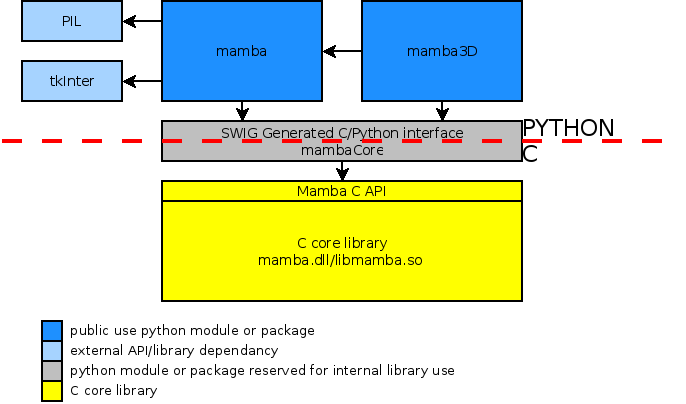
\includegraphics[scale=0.5]{figures/archi.png}
\caption{Library architecture layout}
\label{fig:archi_lay}
\end{figure}

As you already know, Mamba is programmed in C and Python. The C code implements
very basic functions. They are coded to be specific, fast and simple. Each 
function performs only one operation and do it the best it can. The C code is 
compiled to create the core library which is a collection of simple operations.

Simple Wrapper Interface Generator (SWIG) is used to create the interface 
between the C code and the Python code. This tool makes it easier to add new
functions inside the C part by automatically generating the Python wrapper
around it (Except for particular parameters).

The Python code is split into various packages. The mamba package is the 
main package. It implements the imageMb class that is the
central data structure of the library. This class is an extended, more Python
friendly, version of the data structure used to represent image data inside the
C core library. The mamba module also wraps the core functions to simplify them
and make them compatible with the imageMb class.

Because the C core library does not offer functions to read image files, Mamba
relies on the Python Imaging Library (PIL) to do so. An internal module is used
to create an interface to PIL that makes sure images are properly loaded and
converted to a format that is compatible with Mamba internal data representation.

The display capability is implemented by an internal module which relies on
Tkinter for windows and widgets creation.

This architecture is described in figure \ref{fig:archi_lay}.

\subsection{Creating your own display}
\label{cha:create_own_disp}

If your intent is to create your own display for Mamba image, you can create
a "displayer" class inheriting from the mambaDisplayer class described in the
mambaDisplay module. This class is actually an abstract class (or as close
as an abstract class that is allowed by Python). The mambaDisplay module
actually implements one child class of the mambaDisplayer called \_MbDisplayer.
Creating your own display will then look like this:

\lstset{language=Python}
\begin{lstlisting}
import mambaDisplay

# your own displayer (inherits from the generic displayer)
class YourOwnDisplayer(mambaDisplay.mambaDisplayer):
    ...
    
# Creating an instance of your displayer
your_displayer = YourOwnDisplayer()

# Creating an image using your own display rather than the default one
im = imageMb(displayer=your_displayer)

# Or alternatively you could override the getDisplayer function of the 
# mambaDisplay module so that every created image will then use your display
# without having to precise it
def getDisplayer():
    global your_displayer
    return your_displayer
\end{lstlisting}

A "displayer" must implement various functionnalities to work correctly. The 
best way to create your own is to have a look at the default one in mambaDisplay.

You can also create your own display for 3D images and make image3DMb objects
use it.

To create your own 3D display, use the image3DDisplay class as a reference. Your
display will have to offer the methods it describes to work with Mamba3D
images. This class can be found in module display3D of the mamba3D package.

Once you have created your display, you can make image3DMb use it by calling the
constructor with an extra argument:

\lstset{language=Python}
\begin{lstlisting}
# Registering your display at image creation
im3D = image3DMb(displayer=yourDisplayClass)

# Now when you call the showDisplay method, it is your display which is 
# created by default (if no other display was created before).
im3D.show()
# You can force the creation of your display like this.
im3D.show("USR")
\end{lstlisting}

\subsection{Vectorization}
\label{cha:vectorization}

Mamba C core library use vectorized computations to squeeze out better 
performance from your computer. Vectorization is achieved through the SSE2
instruction set available on all modern intel and AMD CPUs.

If you are planning to compile Mamba for other architectures you might want to
use the available equivalent instruction set. You can easily do this by modifying
the file mambaApi\_vector.h found in the src/mambaApi/include-private directory
in the sources.

Replace or add your own definition of the macros MB\_vec* using the appropriate
instruction set.

\subsection{Adding your own 3D grid}
\label{cha:create_grid3D}

To add your own grid, we recommand you have a look at the grids3D module in
the mamba3D package.

In it, you will find a class called \_grid3D that defines all the requested
methods that a grid must define to properly work in Mamba3D. Your own grid
will have to inherit from this class.

Of course, the best way to create your own grid is to copy and modify one
of the aforementioned grids (They can also be found in the grids3D module).

\subsection{Testing Mamba}
\label{cha:testing_mamba}

Mamba has a comprehensive set of tests designed to verify the appropriate
working of the library.

If you made some modifications on the library you may find useful to retest it
to prevent any unwanted regressions or to verify your modification did not break
the library.

Tests are located in the directory test of the sources. You can run the complete
set of test by typing the following command in a terminal:

\texttt{python runTest.py -c -o test\_run.html -v 2}

Once the tests are done, you will find an HTML report with all the results in it.

The test runner make use of coverage (see \url{https://pypi.python.org/pypi/coverage/3.7.1})
package to generate coverage information for the python packages.

If you want more information regarding the test runner, you can type:

\texttt{python runTest.py -h}

\pagebreak

\appendix

\section{To go further}
\label{cha:to_go_further}
\subsection{Python websites}

Here is a list of Python related websites:

\begin{itemize}
\item \url{http://www.python.org}: The official Python website. You can download
it there, find documentation and other links for Python.
\item \url{http://docs.python.org/tutorial/}: The official Python tutorial.
\item \url{http://www.greenteapress.com/thinkpython/thinkCSpy/}: How to Think 
Like a Computer Scientist. A free book to learn computer science with Python
programming. Many translation are available.
\item \url{http://www.pythonware.com/products/pil/}: The Python Imaging Library
website. You can download it, find documentation and source.
\item \url{http://wiki.python.org/moin/TkInter}: A wiki providing ressources
for the Tkinter library used in Mamba for display.
\item \url{http://www.pythonchallenge.com/}: An online puzzle game where you
will need to use Python to solve the riddles.
\end{itemize}

\subsection{Mathematical Morphology websites}

The list below presents websites where you will find courses, documentation and
other information related to mathematical morphology at large:

\begin{itemize}
\item \url{http://cmm.ensmp.fr/}: The Centre de Morphologie Math\'{e}matique
website. This Mines Paristech research laboratory was founded by Georges Matheron 
and Jean Serra, the pioneers of mathematical
morphology. Various publications are available with online courses.
\item \url{http://en.wikipedia.org/wiki/Mathematical_morphology}: The Wikipedia
page on mathematical morphology.
\end{itemize}

\subsection{Other mathematical morphology libraries}

If you are not happy with Mamba, here is a list of other mathematical morphology
libraries:

\begin{itemize}
\item \textsc{\textbf{Fulguro}}: A free library, released under LGPL, implementing
mathematical morphology and images processing functions. Coded in C with wrappers
for Python and Ruby. You can find it at \url{http://fulguro.sourceforge.net/}.
\item \textsc{\textbf{Morph-M}}: A proprietary library developed by the Centre
de Morphologie Math\'{e}matique. Morph-M is coded in C++ with a wrapper for
Python. More information can be found at \url{http://cmm.ensmp.fr/Morph-M/index_en.html}.
\end{itemize}

\end{document}
